\documentclass{article} % For LaTeX2e
\usepackage{iclr2022_conference,times}
\usepackage[utf8]{inputenc}
\usepackage{array}

% Optional math commands from https://github.com/goodfeli/dlbook_notation.
%%%%% NEW MATH DEFINITIONS %%%%%

\usepackage{amsmath,amsfonts,bm}

% Mark sections of captions for referring to divisions of figures
\newcommand{\figleft}{{\em (Left)}}
\newcommand{\figcenter}{{\em (Center)}}
\newcommand{\figright}{{\em (Right)}}
\newcommand{\figtop}{{\em (Top)}}
\newcommand{\figbottom}{{\em (Bottom)}}
\newcommand{\captiona}{{\em (a)}}
\newcommand{\captionb}{{\em (b)}}
\newcommand{\captionc}{{\em (c)}}
\newcommand{\captiond}{{\em (d)}}

% Highlight a newly defined term
\newcommand{\newterm}[1]{{\bf #1}}


% Figure reference, lower-case.
\def\figref#1{figure~\ref{#1}}
% Figure reference, capital. For start of sentence
\def\Figref#1{Figure~\ref{#1}}
\def\twofigref#1#2{figures \ref{#1} and \ref{#2}}
\def\quadfigref#1#2#3#4{figures \ref{#1}, \ref{#2}, \ref{#3} and \ref{#4}}
% Section reference, lower-case.
\def\secref#1{section~\ref{#1}}
% Section reference, capital.
\def\Secref#1{Section~\ref{#1}}
% Reference to two sections.
\def\twosecrefs#1#2{sections \ref{#1} and \ref{#2}}
% Reference to three sections.
\def\secrefs#1#2#3{sections \ref{#1}, \ref{#2} and \ref{#3}}
% Reference to an equation, lower-case.
\def\eqref#1{equation~\ref{#1}}
% Reference to an equation, upper case
\def\Eqref#1{Equation~\ref{#1}}
% A raw reference to an equation---avoid using if possible
\def\plaineqref#1{\ref{#1}}
% Reference to a chapter, lower-case.
\def\chapref#1{chapter~\ref{#1}}
% Reference to an equation, upper case.
\def\Chapref#1{Chapter~\ref{#1}}
% Reference to a range of chapters
\def\rangechapref#1#2{chapters\ref{#1}--\ref{#2}}
% Reference to an algorithm, lower-case.
\def\algref#1{algorithm~\ref{#1}}
% Reference to an algorithm, upper case.
\def\Algref#1{Algorithm~\ref{#1}}
\def\twoalgref#1#2{algorithms \ref{#1} and \ref{#2}}
\def\Twoalgref#1#2{Algorithms \ref{#1} and \ref{#2}}
% Reference to a part, lower case
\def\partref#1{part~\ref{#1}}
% Reference to a part, upper case
\def\Partref#1{Part~\ref{#1}}
\def\twopartref#1#2{parts \ref{#1} and \ref{#2}}

\def\ceil#1{\lceil #1 \rceil}
\def\floor#1{\lfloor #1 \rfloor}
\def\1{\bm{1}}
\newcommand{\train}{\mathcal{D}}
\newcommand{\valid}{\mathcal{D_{\mathrm{valid}}}}
\newcommand{\test}{\mathcal{D_{\mathrm{test}}}}

\def\eps{{\epsilon}}


% Random variables
\def\reta{{\textnormal{$\eta$}}}
\def\ra{{\textnormal{a}}}
\def\rb{{\textnormal{b}}}
\def\rc{{\textnormal{c}}}
\def\rd{{\textnormal{d}}}
\def\re{{\textnormal{e}}}
\def\rf{{\textnormal{f}}}
\def\rg{{\textnormal{g}}}
\def\rh{{\textnormal{h}}}
\def\ri{{\textnormal{i}}}
\def\rj{{\textnormal{j}}}
\def\rk{{\textnormal{k}}}
\def\rl{{\textnormal{l}}}
% rm is already a command, just don't name any random variables m
\def\rn{{\textnormal{n}}}
\def\ro{{\textnormal{o}}}
\def\rp{{\textnormal{p}}}
\def\rq{{\textnormal{q}}}
\def\rr{{\textnormal{r}}}
\def\rs{{\textnormal{s}}}
\def\rt{{\textnormal{t}}}
\def\ru{{\textnormal{u}}}
\def\rv{{\textnormal{v}}}
\def\rw{{\textnormal{w}}}
\def\rx{{\textnormal{x}}}
\def\ry{{\textnormal{y}}}
\def\rz{{\textnormal{z}}}

% Random vectors
\def\rvepsilon{{\mathbf{\epsilon}}}
\def\rvtheta{{\mathbf{\theta}}}
\def\rva{{\mathbf{a}}}
\def\rvb{{\mathbf{b}}}
\def\rvc{{\mathbf{c}}}
\def\rvd{{\mathbf{d}}}
\def\rve{{\mathbf{e}}}
\def\rvf{{\mathbf{f}}}
\def\rvg{{\mathbf{g}}}
\def\rvh{{\mathbf{h}}}
\def\rvu{{\mathbf{i}}}
\def\rvj{{\mathbf{j}}}
\def\rvk{{\mathbf{k}}}
\def\rvl{{\mathbf{l}}}
\def\rvm{{\mathbf{m}}}
\def\rvn{{\mathbf{n}}}
\def\rvo{{\mathbf{o}}}
\def\rvp{{\mathbf{p}}}
\def\rvq{{\mathbf{q}}}
\def\rvr{{\mathbf{r}}}
\def\rvs{{\mathbf{s}}}
\def\rvt{{\mathbf{t}}}
\def\rvu{{\mathbf{u}}}
\def\rvv{{\mathbf{v}}}
\def\rvw{{\mathbf{w}}}
\def\rvx{{\mathbf{x}}}
\def\rvy{{\mathbf{y}}}
\def\rvz{{\mathbf{z}}}

% Elements of random vectors
\def\erva{{\textnormal{a}}}
\def\ervb{{\textnormal{b}}}
\def\ervc{{\textnormal{c}}}
\def\ervd{{\textnormal{d}}}
\def\erve{{\textnormal{e}}}
\def\ervf{{\textnormal{f}}}
\def\ervg{{\textnormal{g}}}
\def\ervh{{\textnormal{h}}}
\def\ervi{{\textnormal{i}}}
\def\ervj{{\textnormal{j}}}
\def\ervk{{\textnormal{k}}}
\def\ervl{{\textnormal{l}}}
\def\ervm{{\textnormal{m}}}
\def\ervn{{\textnormal{n}}}
\def\ervo{{\textnormal{o}}}
\def\ervp{{\textnormal{p}}}
\def\ervq{{\textnormal{q}}}
\def\ervr{{\textnormal{r}}}
\def\ervs{{\textnormal{s}}}
\def\ervt{{\textnormal{t}}}
\def\ervu{{\textnormal{u}}}
\def\ervv{{\textnormal{v}}}
\def\ervw{{\textnormal{w}}}
\def\ervx{{\textnormal{x}}}
\def\ervy{{\textnormal{y}}}
\def\ervz{{\textnormal{z}}}

% Random matrices
\def\rmA{{\mathbf{A}}}
\def\rmB{{\mathbf{B}}}
\def\rmC{{\mathbf{C}}}
\def\rmD{{\mathbf{D}}}
\def\rmE{{\mathbf{E}}}
\def\rmF{{\mathbf{F}}}
\def\rmG{{\mathbf{G}}}
\def\rmH{{\mathbf{H}}}
\def\rmI{{\mathbf{I}}}
\def\rmJ{{\mathbf{J}}}
\def\rmK{{\mathbf{K}}}
\def\rmL{{\mathbf{L}}}
\def\rmM{{\mathbf{M}}}
\def\rmN{{\mathbf{N}}}
\def\rmO{{\mathbf{O}}}
\def\rmP{{\mathbf{P}}}
\def\rmQ{{\mathbf{Q}}}
\def\rmR{{\mathbf{R}}}
\def\rmS{{\mathbf{S}}}
\def\rmT{{\mathbf{T}}}
\def\rmU{{\mathbf{U}}}
\def\rmV{{\mathbf{V}}}
\def\rmW{{\mathbf{W}}}
\def\rmX{{\mathbf{X}}}
\def\rmY{{\mathbf{Y}}}
\def\rmZ{{\mathbf{Z}}}

% Elements of random matrices
\def\ermA{{\textnormal{A}}}
\def\ermB{{\textnormal{B}}}
\def\ermC{{\textnormal{C}}}
\def\ermD{{\textnormal{D}}}
\def\ermE{{\textnormal{E}}}
\def\ermF{{\textnormal{F}}}
\def\ermG{{\textnormal{G}}}
\def\ermH{{\textnormal{H}}}
\def\ermI{{\textnormal{I}}}
\def\ermJ{{\textnormal{J}}}
\def\ermK{{\textnormal{K}}}
\def\ermL{{\textnormal{L}}}
\def\ermM{{\textnormal{M}}}
\def\ermN{{\textnormal{N}}}
\def\ermO{{\textnormal{O}}}
\def\ermP{{\textnormal{P}}}
\def\ermQ{{\textnormal{Q}}}
\def\ermR{{\textnormal{R}}}
\def\ermS{{\textnormal{S}}}
\def\ermT{{\textnormal{T}}}
\def\ermU{{\textnormal{U}}}
\def\ermV{{\textnormal{V}}}
\def\ermW{{\textnormal{W}}}
\def\ermX{{\textnormal{X}}}
\def\ermY{{\textnormal{Y}}}
\def\ermZ{{\textnormal{Z}}}

% Vectors
\def\vzero{{\bm{0}}}
\def\vone{{\bm{1}}}
\def\vmu{{\bm{\mu}}}
\def\vtheta{{\bm{\theta}}}
\def\va{{\bm{a}}}
\def\vb{{\bm{b}}}
\def\vc{{\bm{c}}}
\def\vd{{\bm{d}}}
\def\ve{{\bm{e}}}
\def\vf{{\bm{f}}}
\def\vg{{\bm{g}}}
\def\vh{{\bm{h}}}
\def\vi{{\bm{i}}}
\def\vj{{\bm{j}}}
\def\vk{{\bm{k}}}
\def\vl{{\bm{l}}}
\def\vm{{\bm{m}}}
\def\vn{{\bm{n}}}
\def\vo{{\bm{o}}}
\def\vp{{\bm{p}}}
\def\vq{{\bm{q}}}
\def\vr{{\bm{r}}}
\def\vs{{\bm{s}}}
\def\vt{{\bm{t}}}
\def\vu{{\bm{u}}}
\def\vv{{\bm{v}}}
\def\vw{{\bm{w}}}
\def\vx{{\bm{x}}}
\def\vy{{\bm{y}}}
\def\vz{{\bm{z}}}

% Elements of vectors
\def\evalpha{{\alpha}}
\def\evbeta{{\beta}}
\def\evepsilon{{\epsilon}}
\def\evlambda{{\lambda}}
\def\evomega{{\omega}}
\def\evmu{{\mu}}
\def\evpsi{{\psi}}
\def\evsigma{{\sigma}}
\def\evtheta{{\theta}}
\def\eva{{a}}
\def\evb{{b}}
\def\evc{{c}}
\def\evd{{d}}
\def\eve{{e}}
\def\evf{{f}}
\def\evg{{g}}
\def\evh{{h}}
\def\evi{{i}}
\def\evj{{j}}
\def\evk{{k}}
\def\evl{{l}}
\def\evm{{m}}
\def\evn{{n}}
\def\evo{{o}}
\def\evp{{p}}
\def\evq{{q}}
\def\evr{{r}}
\def\evs{{s}}
\def\evt{{t}}
\def\evu{{u}}
\def\evv{{v}}
\def\evw{{w}}
\def\evx{{x}}
\def\evy{{y}}
\def\evz{{z}}

% Matrix
\def\mA{{\bm{A}}}
\def\mB{{\bm{B}}}
\def\mC{{\bm{C}}}
\def\mD{{\bm{D}}}
\def\mE{{\bm{E}}}
\def\mF{{\bm{F}}}
\def\mG{{\bm{G}}}
\def\mH{{\bm{H}}}
\def\mI{{\bm{I}}}
\def\mJ{{\bm{J}}}
\def\mK{{\bm{K}}}
\def\mL{{\bm{L}}}
\def\mM{{\bm{M}}}
\def\mN{{\bm{N}}}
\def\mO{{\bm{O}}}
\def\mP{{\bm{P}}}
\def\mQ{{\bm{Q}}}
\def\mR{{\bm{R}}}
\def\mS{{\bm{S}}}
\def\mT{{\bm{T}}}
\def\mU{{\bm{U}}}
\def\mV{{\bm{V}}}
\def\mW{{\bm{W}}}
\def\mX{{\bm{X}}}
\def\mY{{\bm{Y}}}
\def\mZ{{\bm{Z}}}
\def\mBeta{{\bm{\beta}}}
\def\mPhi{{\bm{\Phi}}}
\def\mLambda{{\bm{\Lambda}}}
\def\mSigma{{\bm{\Sigma}}}

% Tensor
\DeclareMathAlphabet{\mathsfit}{\encodingdefault}{\sfdefault}{m}{sl}
\SetMathAlphabet{\mathsfit}{bold}{\encodingdefault}{\sfdefault}{bx}{n}
\newcommand{\tens}[1]{\bm{\mathsfit{#1}}}
\def\tA{{\tens{A}}}
\def\tB{{\tens{B}}}
\def\tC{{\tens{C}}}
\def\tD{{\tens{D}}}
\def\tE{{\tens{E}}}
\def\tF{{\tens{F}}}
\def\tG{{\tens{G}}}
\def\tH{{\tens{H}}}
\def\tI{{\tens{I}}}
\def\tJ{{\tens{J}}}
\def\tK{{\tens{K}}}
\def\tL{{\tens{L}}}
\def\tM{{\tens{M}}}
\def\tN{{\tens{N}}}
\def\tO{{\tens{O}}}
\def\tP{{\tens{P}}}
\def\tQ{{\tens{Q}}}
\def\tR{{\tens{R}}}
\def\tS{{\tens{S}}}
\def\tT{{\tens{T}}}
\def\tU{{\tens{U}}}
\def\tV{{\tens{V}}}
\def\tW{{\tens{W}}}
\def\tX{{\tens{X}}}
\def\tY{{\tens{Y}}}
\def\tZ{{\tens{Z}}}


% Graph
\def\gA{{\mathcal{A}}}
\def\gB{{\mathcal{B}}}
\def\gC{{\mathcal{C}}}
\def\gD{{\mathcal{D}}}
\def\gE{{\mathcal{E}}}
\def\gF{{\mathcal{F}}}
\def\gG{{\mathcal{G}}}
\def\gH{{\mathcal{H}}}
\def\gI{{\mathcal{I}}}
\def\gJ{{\mathcal{J}}}
\def\gK{{\mathcal{K}}}
\def\gL{{\mathcal{L}}}
\def\gM{{\mathcal{M}}}
\def\gN{{\mathcal{N}}}
\def\gO{{\mathcal{O}}}
\def\gP{{\mathcal{P}}}
\def\gQ{{\mathcal{Q}}}
\def\gR{{\mathcal{R}}}
\def\gS{{\mathcal{S}}}
\def\gT{{\mathcal{T}}}
\def\gU{{\mathcal{U}}}
\def\gV{{\mathcal{V}}}
\def\gW{{\mathcal{W}}}
\def\gX{{\mathcal{X}}}
\def\gY{{\mathcal{Y}}}
\def\gZ{{\mathcal{Z}}}

% Sets
\def\sA{{\mathbb{A}}}
\def\sB{{\mathbb{B}}}
\def\sC{{\mathbb{C}}}
\def\sD{{\mathbb{D}}}
% Don't use a set called E, because this would be the same as our symbol
% for expectation.
\def\sF{{\mathbb{F}}}
\def\sG{{\mathbb{G}}}
\def\sH{{\mathbb{H}}}
\def\sI{{\mathbb{I}}}
\def\sJ{{\mathbb{J}}}
\def\sK{{\mathbb{K}}}
\def\sL{{\mathbb{L}}}
\def\sM{{\mathbb{M}}}
\def\sN{{\mathbb{N}}}
\def\sO{{\mathbb{O}}}
\def\sP{{\mathbb{P}}}
\def\sQ{{\mathbb{Q}}}
\def\sR{{\mathbb{R}}}
\def\sS{{\mathbb{S}}}
\def\sT{{\mathbb{T}}}
\def\sU{{\mathbb{U}}}
\def\sV{{\mathbb{V}}}
\def\sW{{\mathbb{W}}}
\def\sX{{\mathbb{X}}}
\def\sY{{\mathbb{Y}}}
\def\sZ{{\mathbb{Z}}}

% Entries of a matrix
\def\emLambda{{\Lambda}}
\def\emA{{A}}
\def\emB{{B}}
\def\emC{{C}}
\def\emD{{D}}
\def\emE{{E}}
\def\emF{{F}}
\def\emG{{G}}
\def\emH{{H}}
\def\emI{{I}}
\def\emJ{{J}}
\def\emK{{K}}
\def\emL{{L}}
\def\emM{{M}}
\def\emN{{N}}
\def\emO{{O}}
\def\emP{{P}}
\def\emQ{{Q}}
\def\emR{{R}}
\def\emS{{S}}
\def\emT{{T}}
\def\emU{{U}}
\def\emV{{V}}
\def\emW{{W}}
\def\emX{{X}}
\def\emY{{Y}}
\def\emZ{{Z}}
\def\emSigma{{\Sigma}}

% entries of a tensor
% Same font as tensor, without \bm wrapper
\newcommand{\etens}[1]{\mathsfit{#1}}
\def\etLambda{{\etens{\Lambda}}}
\def\etA{{\etens{A}}}
\def\etB{{\etens{B}}}
\def\etC{{\etens{C}}}
\def\etD{{\etens{D}}}
\def\etE{{\etens{E}}}
\def\etF{{\etens{F}}}
\def\etG{{\etens{G}}}
\def\etH{{\etens{H}}}
\def\etI{{\etens{I}}}
\def\etJ{{\etens{J}}}
\def\etK{{\etens{K}}}
\def\etL{{\etens{L}}}
\def\etM{{\etens{M}}}
\def\etN{{\etens{N}}}
\def\etO{{\etens{O}}}
\def\etP{{\etens{P}}}
\def\etQ{{\etens{Q}}}
\def\etR{{\etens{R}}}
\def\etS{{\etens{S}}}
\def\etT{{\etens{T}}}
\def\etU{{\etens{U}}}
\def\etV{{\etens{V}}}
\def\etW{{\etens{W}}}
\def\etX{{\etens{X}}}
\def\etY{{\etens{Y}}}
\def\etZ{{\etens{Z}}}

% The true underlying data generating distribution
\newcommand{\pdata}{p_{\rm{data}}}
% The empirical distribution defined by the training set
\newcommand{\ptrain}{\hat{p}_{\rm{data}}}
\newcommand{\Ptrain}{\hat{P}_{\rm{data}}}
% The model distribution
\newcommand{\pmodel}{p_{\rm{model}}}
\newcommand{\Pmodel}{P_{\rm{model}}}
\newcommand{\ptildemodel}{\tilde{p}_{\rm{model}}}
% Stochastic autoencoder distributions
\newcommand{\pencode}{p_{\rm{encoder}}}
\newcommand{\pdecode}{p_{\rm{decoder}}}
\newcommand{\precons}{p_{\rm{reconstruct}}}

\newcommand{\laplace}{\mathrm{Laplace}} % Laplace distribution

\newcommand{\E}{\mathbb{E}}
\newcommand{\Ls}{\mathcal{L}}
\newcommand{\R}{\mathbb{R}}
\newcommand{\emp}{\tilde{p}}
\newcommand{\lr}{\alpha}
\newcommand{\reg}{\lambda}
\newcommand{\rect}{\mathrm{rectifier}}
\newcommand{\softmax}{\mathrm{softmax}}
\newcommand{\sigmoid}{\sigma}
\newcommand{\softplus}{\zeta}
\newcommand{\KL}{D_{\mathrm{KL}}}
\newcommand{\Var}{\mathrm{Var}}
\newcommand{\standarderror}{\mathrm{SE}}
\newcommand{\Cov}{\mathrm{Cov}}
% Wolfram Mathworld says $L^2$ is for function spaces and $\ell^2$ is for vectors
% But then they seem to use $L^2$ for vectors throughout the site, and so does
% wikipedia.
\newcommand{\normlzero}{L^0}
\newcommand{\normlone}{L^1}
\newcommand{\normltwo}{L^2}
\newcommand{\normlp}{L^p}
\newcommand{\normmax}{L^\infty}

\newcommand{\parents}{Pa} % See usage in notation.tex. Chosen to match Daphne's book.

\DeclareMathOperator*{\argmax}{arg\,max}
\DeclareMathOperator*{\argmin}{arg\,min}

\DeclareMathOperator{\sign}{sign}
\DeclareMathOperator{\Tr}{Tr}
\let\ab\allowbreak


%######## APS360: Uncomment your submission name
\newcommand{\apsname}{Project Proposal}
%\newcommand{\apsname}{Progress Report}
%\newcommand{\apsname}{Final Report}

%######## APS360: Put your Group Number here
\newcommand{\gpnumber}{35}

\usepackage{hyperref}
\usepackage{url}
\usepackage{graphicx}

%######## APS360: Put your project Title here
\title{Let's Beat Geometry Dash  \\ 
APS360 Project Proposal}


%######## APS360: Put your names, student IDs and Emails here
\author{Joel Vadakken  \\
Student\# 10010089798\\
\texttt{j.vadakken@mail.utoronto.ca} \\
\And
Skyler Han  \\
Student\# 1009794830 \\
\texttt{hs.han@mail.utoronto.ca} \\
\AND
Ian Lu  \\
Student\# 1009972139 \\
\texttt{i.lu@mail.utoronto.ca} \\
\And
Jaden Dai \\
Student\# 1009972228 \\
\texttt{jaden.dai@mail.utoronto.ca} \\
\AND
}

% The \author macro works with any number of authors. There are two commands
% used to separate the names and addresses of multiple authors: \And and \AND.
%
% Using \And between authors leaves it to \LaTeX{} to determine where to break
% the lines. Using \AND forces a linebreak at that point. So, if \LaTeX{}
% puts 3 of 4 authors names on the first line, and the last on the second
% line, try using \AND instead of \And before the third author name.

\newcommand{\fix}{\marginpar{FIX}}
\newcommand{\new}{\marginpar{NEW}}

\iclrfinalcopy 
%######## APS360: Document starts here
\begin{document}


\maketitle

\begin{abstract}
Our team's project proposal is to create a bot that can play 
Geometry Dash using machine learning. The bot will be trained
with two architectures, a convoluted neural network so that it
can identify obstacles in the game, and with deep reinforcement
learning so that the bot can learn to make the right choices.
%######## APS360: Do not change the next line. This shows your Main body page count.
----Total Pages: \pageref{last_page}
\end{abstract}



\section{Introduction}

Geometry Dash is a popular platformer video game 
where the player attempts to navigate through 
obstacles in order to reach the end of a level. 
The game features a variety of game modes and 
unique objects.

A video of the first level can be seen here:
\href{https://www.youtube.com/watch?v=bbVEbqU9wPo}{https://www.youtube.com/watch?v=bbVEbqU9wPo} 

The player is controlled by one input which 
determines whether or not the player jumps. 
Our aim is to build an agent that can beat many 
of the game’s levels. This will involve training 
two models. We aim to analyze screen information 
using a CNN architecture to find the positions 
of structures and hazards, then use a deep 
learning reinforcement architecture to determine 
agent behavior.

Our project was inspired by similar work in other
games such as Mario. However, most other games simply 
require you to jump over basic obstacles and do not require 
complex decision making. Geometry Dash is unique and 
interesting because many levels feature “fakes” 
where jumping objects can trick the player into death.
See Fig. \ref{fig:cycles_false_jump_img} for an example. 

\begin{figure}[!h]
\begin{center}
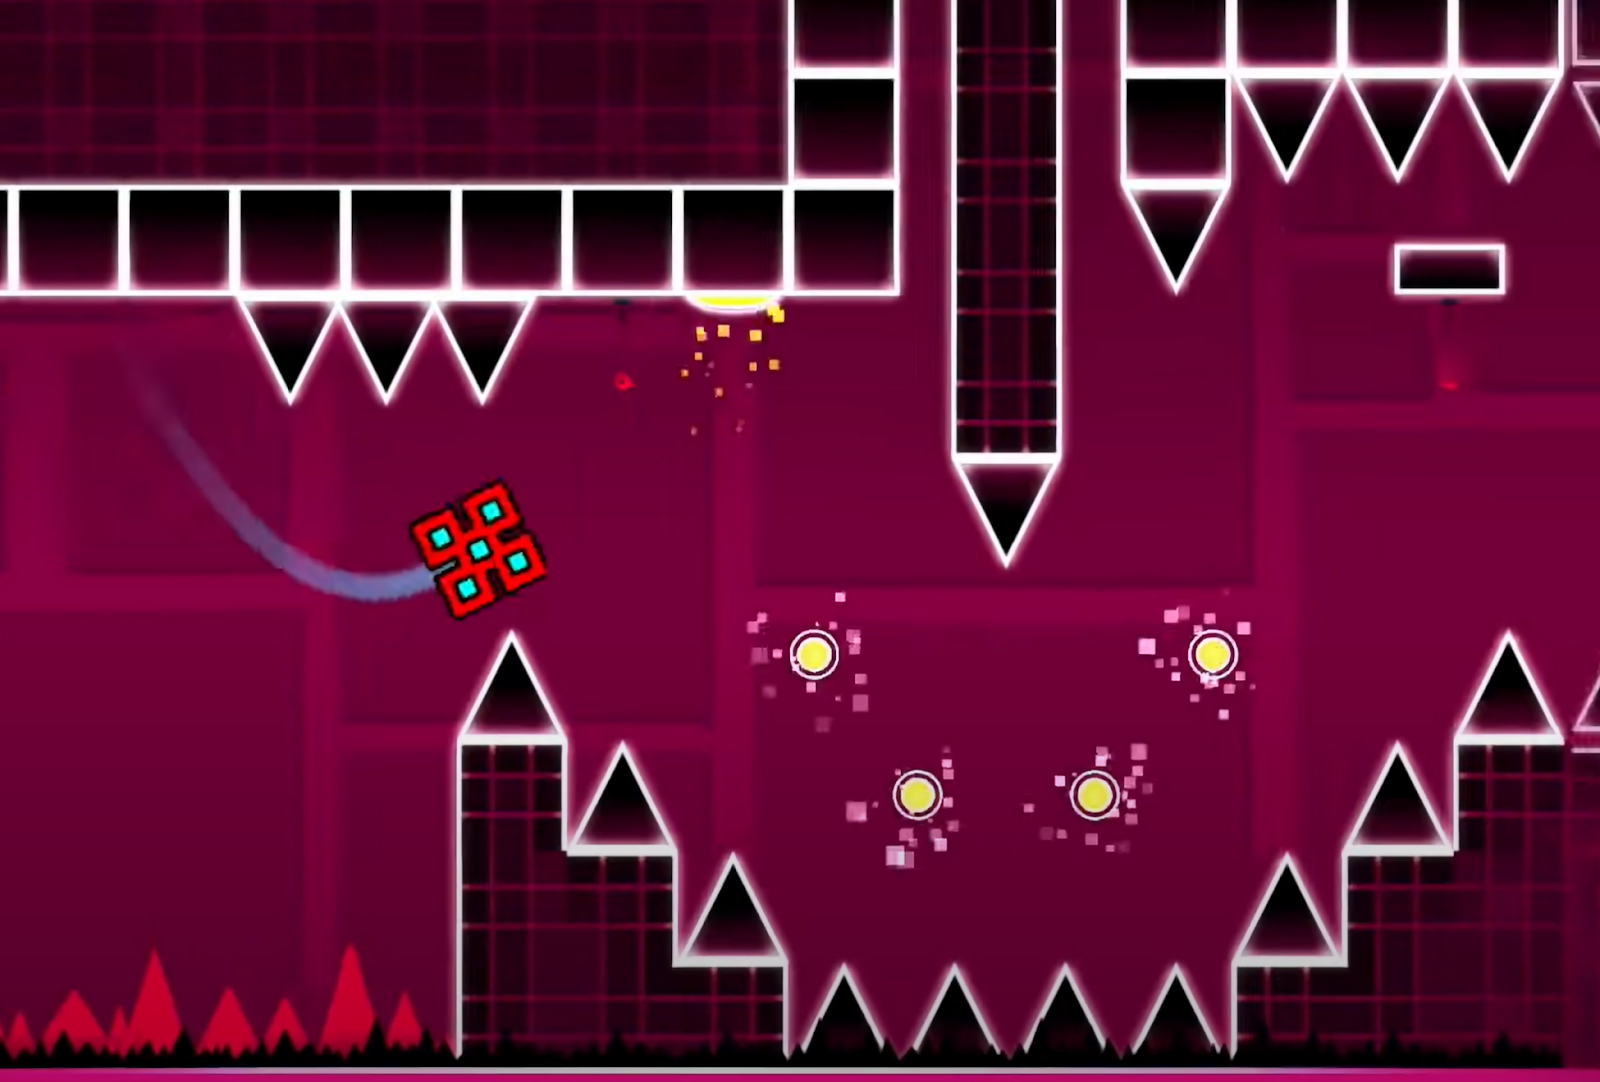
\includegraphics[width=0.6\textwidth]{Figs/GeoDash_Cycles_False_jump.png}
\end{center}
\caption{A screenshot from the 9th level “Cycles”. 
Normally, interacting with the yellow orbs allows the
players to jump higher and avoid obstacles. In this case, 
however, interacting with any of the yellow orbs will result 
in the player losing. \citep{GD+cycles+screenshot}}
\label{fig:cycles_false_jump_img}
\end{figure}

Furthermore, many community-made levels often feature 
intricate designs that may confuse computer systems, as 
can be seen in Fig. \ref{fig:edge_of_destiny} for example.

\begin{figure}[!h]
\begin{center}
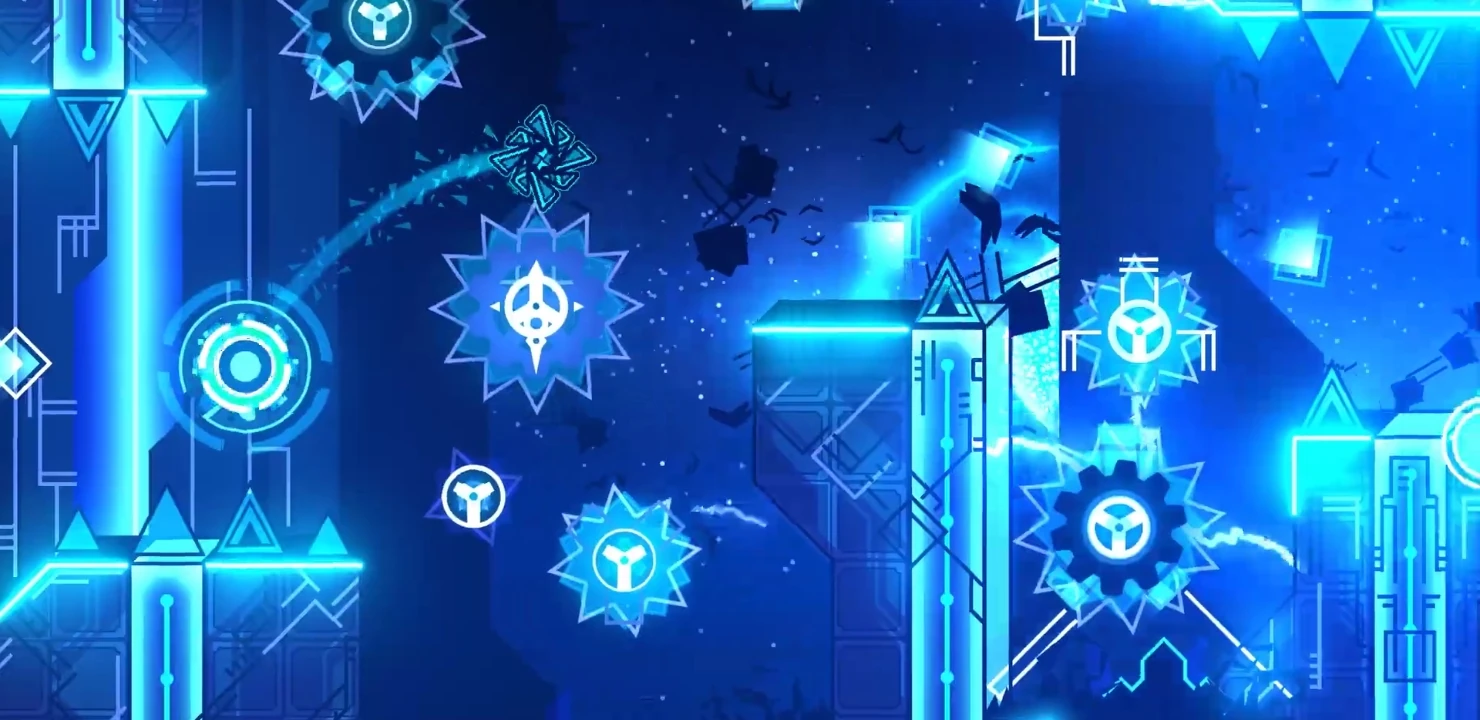
\includegraphics[width=0.6\textwidth]{Figs/GeoDash_Level_ex.png}
\end{center}
\caption{A screenshot from the custom level “Edge of Destiny.” 
Note the intricate details that make it harder to see the hazards. 
\citep{GD+edge_of_destiny}}
\label{fig:edge_of_destiny}
\end{figure}

We believe that a deep-learning approach can enable a computer 
to tackle both these issues through object recognition and avoidance 
of fake objects and routes.

\section{Background and Related Work (4 marks)}


\begin{figure}[!h]
\begin{center}
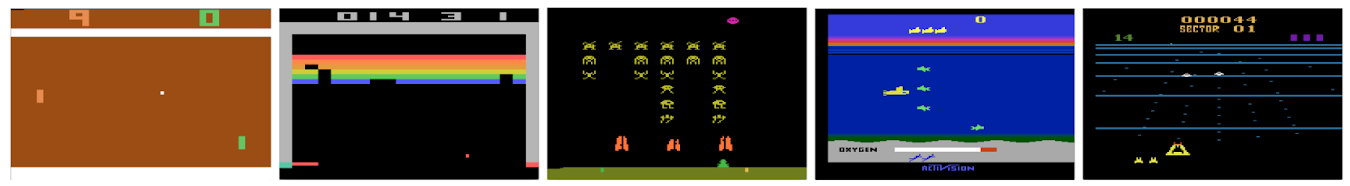
\includegraphics[width=1.0\textwidth]{Figs/Deepmind_atari.png}
\end{center}
\caption{Screenshots from 5 Atari 2600 games: 
(Left-to-right) Pong, Breakout, Space Invaders, Seaquest, Beam Rider
\citep{Playing+Atari+with+Deep+Reinforcement+Learning}}
\label{fig:Deep_mind_Atari_AI}
\end{figure}

The first trial of applying deep reinforcement learning to train a
video game agent originates from a paper written by
\cite{Playing+Atari+with+Deep+Reinforcement+Learning} at 
DeepMind. They created a program that could play Atari games using
deep reinforcement learning. See Fig. \ref{fig:Deep_mind_Atari_AI}
This paper demonstrates that a convolutional neural network can 
overcome the long training process of reinforcement learning to 
learn successful control policies from raw video data in complex 
RL environments. The network is trained with a variant of the 
Q-learning algorithm, with stochastic gradient descent to update 
the weights. And the game agent surpassed an expert human player 
in every game they implemented.

\begin{figure}[!h]
\begin{center}
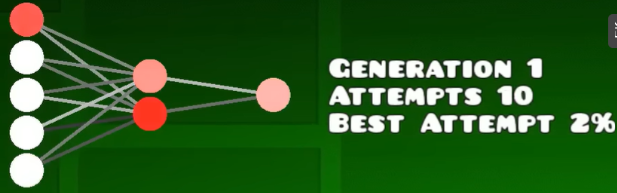
\includegraphics[width=0.8\textwidth]{Figs/CodeNoodlesScreenshot.png}
\end{center}
\caption{A screenshot of CodeNoodle's visualization of his neural network
from his Youtube video. 
\citep{AI+Learns+to+Play+GD}}
\label{fig:Code_Noodles}
\end{figure}

\cite{AI+Learns+to+Play+GD} created a relatively simple 
Neural Network to play Geometry Dash that takes in 
some information (ie. intersection with  “orb” objects, 
distance to blocks, overhead blocks) and outputs an action.
See Fig \ref{fig:Code_Noodles}.
However, we believe 
that this solution is inadequate as it runs on a simplified 
version of Geometry Dash instead of the official game. The 
distance and position of the obstacles are readily available 
information to the model, which would not be the case in the 
real version. Furthermore, the simplistic neural network 
essentially functions as a decision tree, which could fail 
in some cases to the aforementioned misleading objects.

\begin{figure}[!h]
\begin{center}
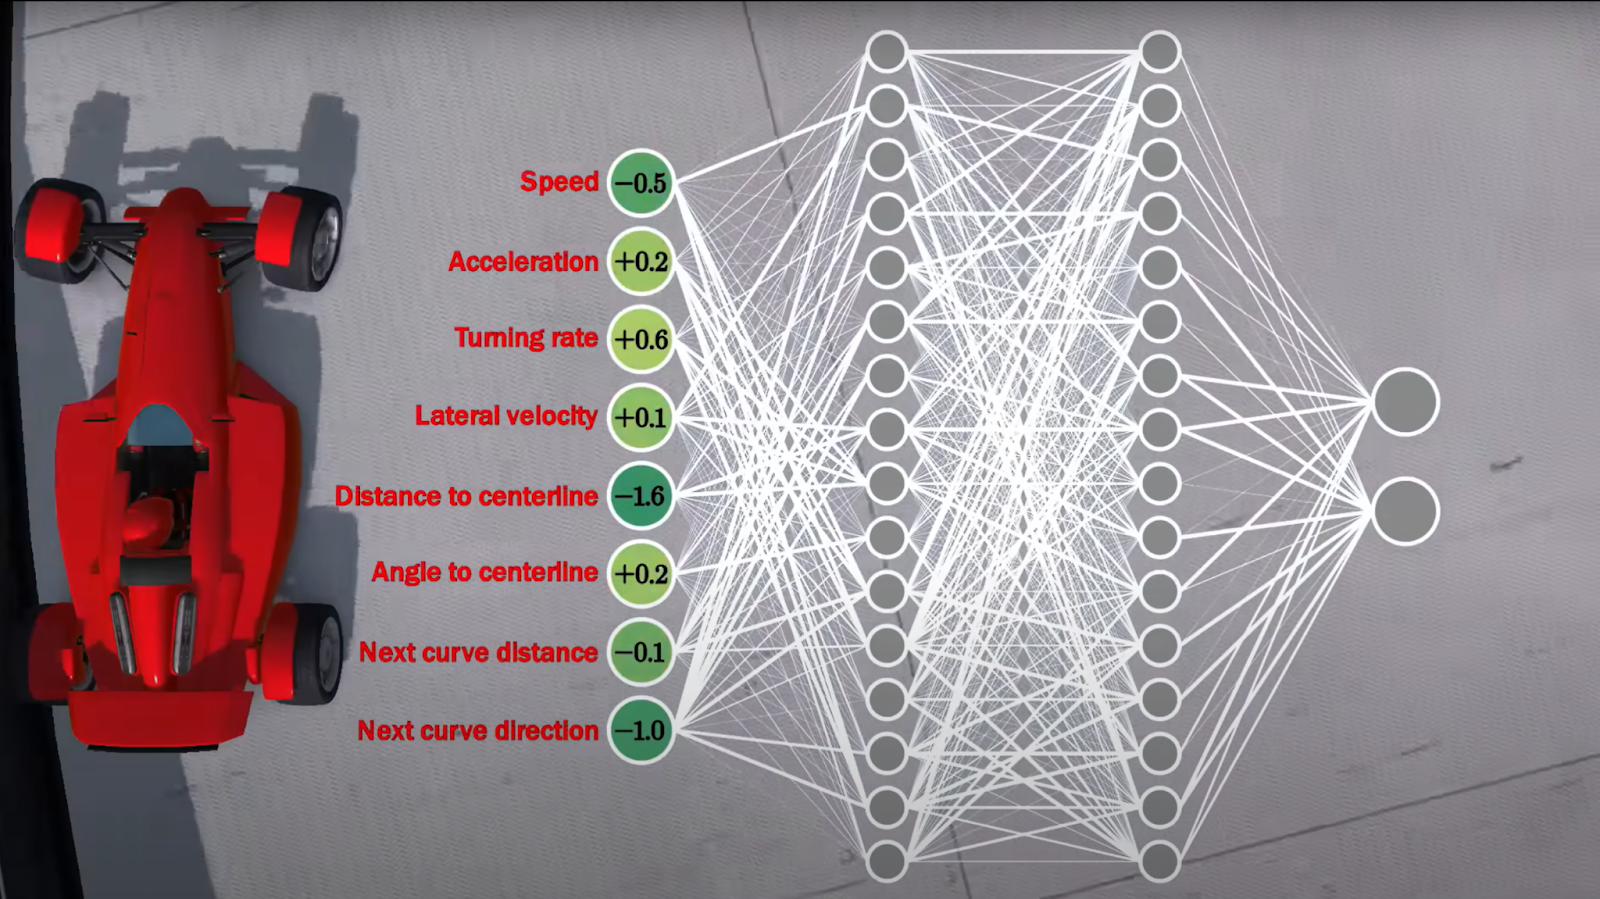
\includegraphics[width=0.8\textwidth]{Figs/Trackmania_AI_neural_network.png}
\end{center}
\caption{A screenshot of Yosh's visualization of his neural network
for his trackmania bot. 
\citep{Trackmania+AI}}
\label{fig:Trackmania_AI}
\end{figure}

\cite{Trackmania+AI} created a Youtube video that demonstrates that 
an AI can come to understand complex in-game physics systems and surpass
human-level performance through training. Trackmania shares a similar 
overarching gameplay system to Geometry Dash in which a player considers 
their environment in order to control their in-game model. Furthermore, both 
games feature fairly complex physics systems. Since the Trackmania AI was 
able to master its game’s physics system, we believe that a similar approach 
applied to Geometry Dash may also give strong performance. See Fig \ref{fig:Trackmania_AI}

\cite{Robot+Object+Avoidance+Method} wrote a paper detailing how 
they split up an image for a robot into a bunch of different segments. 
This might be relevant for us as we could split up the images we attain
from Geometry Dash into an array of squares, and try to sample at a
specific framerate.

\begin{figure}[!h]
\begin{center}
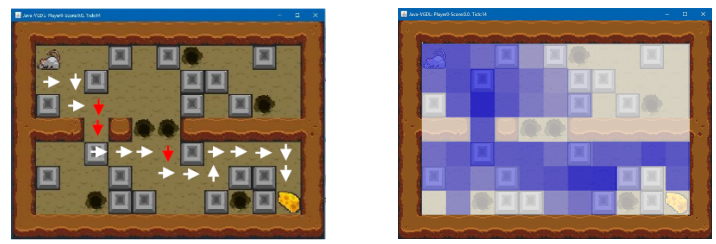
\includegraphics[width=1.0\textwidth]{Figs/Q_Learn_Game.png}
\end{center}
\caption{Video game with optimal path shown (left) vs Deep Q Agent Heat Map 
(right). \citep{General+Video+Game+AI:+Learning+from+Screen+Capture}}
\label{fig:Q_Learn_game}
\end{figure}

\cite{General+Video+Game+AI:+Learning+from+Screen+Capture} wrote a paper that explicitly uses a combination of CNN and Q-learning network to 
train an AI that can play a variety of games. They utilize CNNs to perform 
feature extraction and determine the best course of action, while the Q-
learning component aims to improve decision-making capabilities. They also 
utilize various pre-processing methods (resizing, etc.). Their work 
culminated in an agent that could effectively traverse some 2D environments. This paper showcases how a combination of CNN and Q-learning can enable an 
agent to plan a path through a level, which is fairly similar to what we are 
attempting to achieve. Their techniques may be a useful reference for our own 
project. See Fig \ref{fig:Q_Learn_game}.

\cite{DeepMind+Sima} at Deepmind created a model, called SIMA, 
that can take visual observations from a game to carry out an 
instruction by outputting keyboard events. Although their model does not achieve the same end goal as us (following instruction vs autonomous gameplay), their agent’s ability to understand complex visual information and map it to keyboard inputs supports our approach of utilizing screen capture for object detection and behavior planning. Furthermore, the team’s approach to rewarding and punishing agents may serve as a useful reference for our specific game.

\section{Data Processing (2 marks)}

Our data for our two architectures will both come from the game itself. A CNN 
model will classify the data, and we will use that to create an environment to 
train the RL model. 

In order to identify the types of terrain objects we propose the use of a CNN 
to classify different terrain objects into numerical values in a processed 
tensor that can be passed as an input into the RL model. 

To reduce computational complexity and to preserve the accuracy of the CNN 
classifier, the CNN will include a grayscale filter. Each frame will be grayscale, and the background and each pixel 
will take the value of the mean colour in its associated area such that each 
pixel will consist of one colour value. 

The CNN will be trained on various snapshot frames throughout Geometry Dash 
levels and the corresponding labels for each object terrain in each frame can 
be created using the GD MegaHack v7 mod which identifies the terrain object 
types on a given screen. The CNN will take as an input a single Geometry Dash 
frame, and will output a tensor of the same size with the rgb dimension removed. 
The processed values of the tensor will each be associated with a different 
terrain object in Geometry Dash. Ex: 
\begin{itemize}
\item 0 for air (nothing)
\item 1 for a platform
\item -1 for a spike
\item Some set of integers for portals
\item Some set of integers for orbs
\item Some set of integers for pads
\item Other integers for other game elements
\end{itemize}
The RL model will use the CNN model as it trains in its environment. The tensor 
size of a singular dataset will consist of the number of frames in that geometry 
dash level, the number of pixels on a screen per frame, and their rgb values (number of frames, number 
of pixels to make up a column, number of pixels to make up a row, rgb values). 
The RL model will use this data to output a tensor of size 1 that dictates 
whether 
the bot should jump or not jump. 


\section{Architecture (2 marks)}

\subsection{CNN Model}

\begin{figure}[!htbp]
\begin{center}
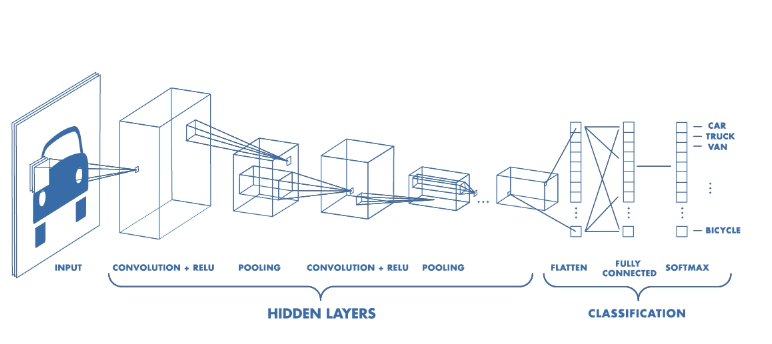
\includegraphics[width=1.0\textwidth]{Figs/CNN_sample_structure.png}
\end{center}
\caption{An example of how a CNN neural network might analyze our data.}
\label{fig:CNN_neural_network}
\end{figure}

We will utilize a CNN to analyze the game screen and find the positions of hazards, platforms, and other interactable objects, such as can be seen in Fig \ref{fig:CNN_neural_network}. A CNN is a type of ANN that retains the geometry of the data and performs convolutions through a kernel with variable parameters that goes across the input (usually a 2D image). This will leverage the CNN architecture’s ability to understand complex shapes and patterns, and will enable accurate positional information that can later be used by the RL agent.

The CNN will be comprised of a set number of layers and will take in as an
input one frame from the game screen (640x480x3 Tensor), and output 
640x480 array of integer values representing different object types.
 

\subsection{Reinforcement Learning Model}

\begin{figure}[!htbp]
\begin{center}
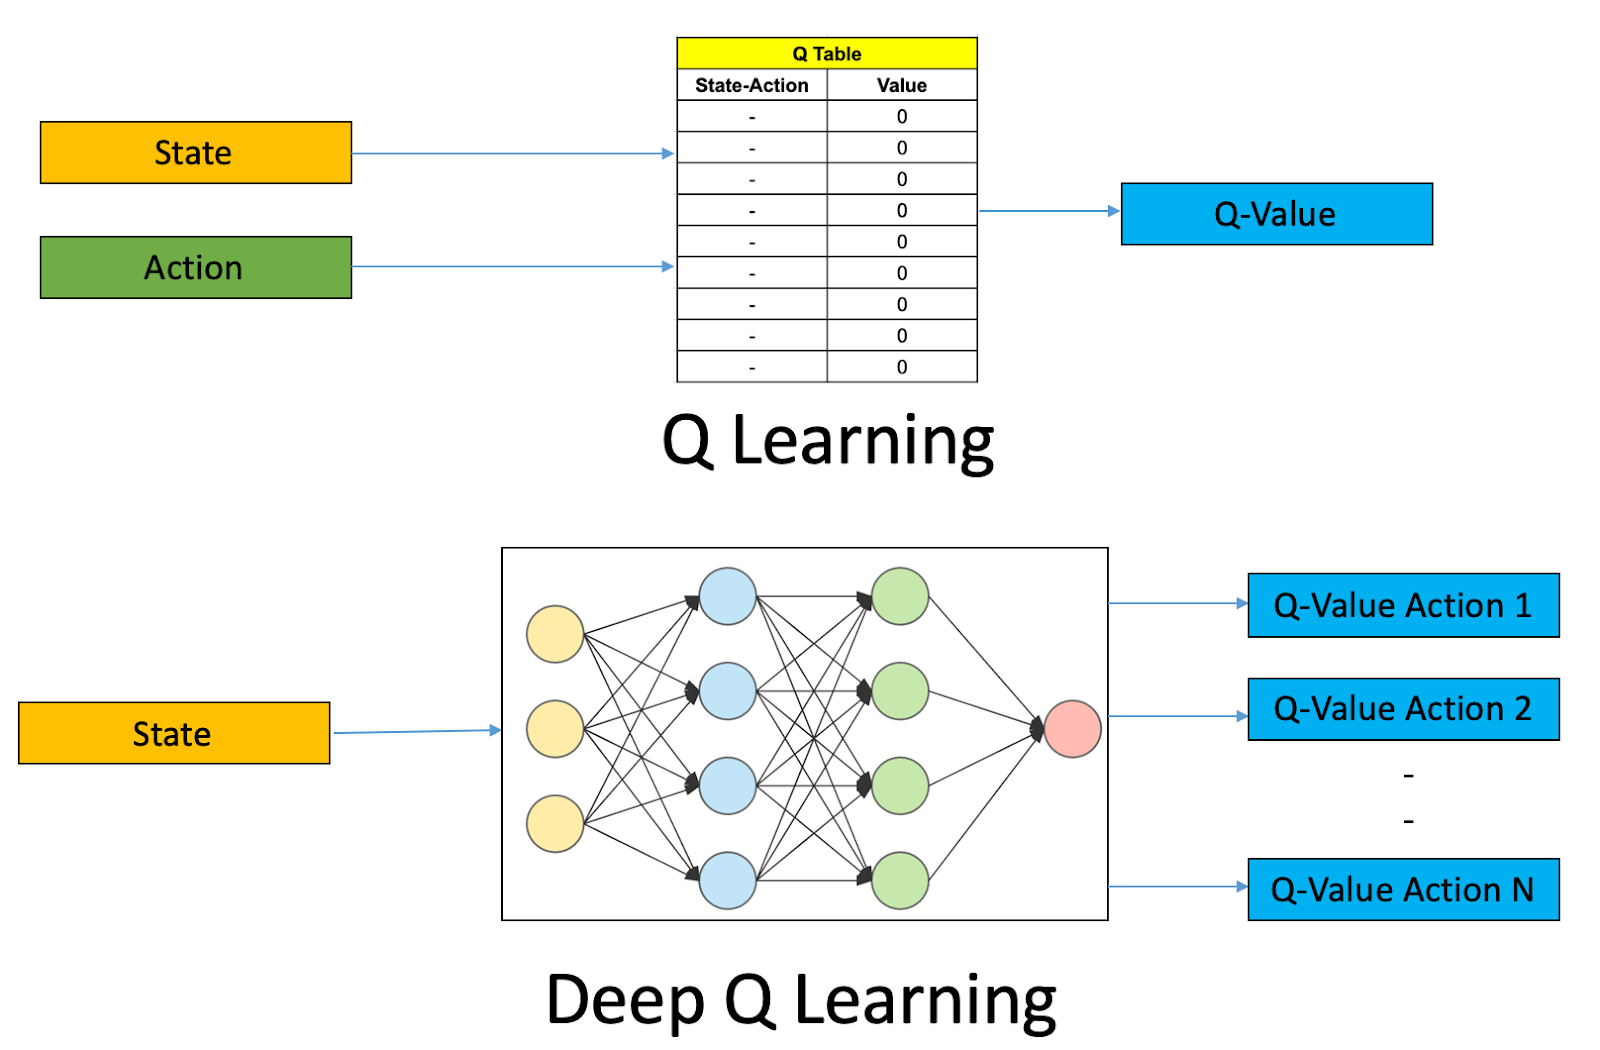
\includegraphics[width=1.0\textwidth]{Figs/QLearn_img.png}
\end{center}
\caption{A flowchart that shows how Deep Q learning is used.}
\label{fig:Deep_Q_Learn}
\end{figure}

We will use a similar reinforcement learning model as was developed by 
\cite{Playing+Atari+with+Deep+Reinforcement+Learning}. This will include
the following:

\begin{itemize}
    \item[\textbf{1.}] \textbf{Environment}
    \begin{itemize}
        \item The Geometry Dash game environment needs to be set up so that it 
        can interact with the agent. 
        \item The environment should provide the current state of the game 
        (e.g., position of the player, obstacles) and allow the agent to perform 
        actions (e.g., jump, no jump).
        \item We would need to build the environment with OpenAI Gym to train 
        the agent since we would need to interact with the RL modules.
    \end{itemize}

    \item[\textbf{2.}] \textbf{State Representation}
    \begin{itemize}
        \item We can get the state from the feedback from the CNN by knowing 
        where the obstacle is in the frame and the position of the player.
    \end{itemize}

    \item[\textbf{3.}] \textbf{Action Space}
    \begin{itemize}
        \item The action space \( A \) consists of discrete actions the agent 
        can take. 
        \item In Geometry Dash, this could be simplified to two actions: jump 
        or no jump.
    \end{itemize}

    \item[\textbf{4.}] \textbf{Replay Memory}
    \begin{itemize}
        \item We store the Geometry Dash agent’s experiences at each time-step, 
        \( e_t = (s_t, a_t, r_t, s_{t+1}) \) in a dataset \( D = \{e_1, \ldots, e_N\} \).
        \item These experiences are pooled over many episodes into a replay memory.
        \item We apply Q-learning updates to a small batch of the samples 
        randomly chosen from the dataset.
    \end{itemize}

    \item[\textbf{5.}] \textbf{Reward Function}
    \begin{itemize}
        \item Define a reward function that provides positive rewards for 
        progress (e.g., distance covered, points scored) and negative rewards 
        for failures (e.g., hitting an obstacle).
    \end{itemize}

    \item[\textbf{6.}] \textbf{Training Procedure}
    \begin{itemize}
        \item Initialize the replay memory \( D \) to a fixed capacity.
        \item Initialize the Q-network with random weights.
        \item For each episode:
        \begin{itemize}
            \item Initialize the starting state \( s_1 \).
            \item For each time-step \( t \):
            \begin{itemize}
                \item With probability \( \epsilon \), select a random action \( a_t \). Otherwise, select \( a_t = \arg\max_a Q(s_t, a; \theta) \).
                \item Execute action \( a_t \) in the game and observe reward \( r_t \) and next state \( s_{t+1} \).
                \item Store experience \( e_t = (s_t, a_t, r_t, s_{t+1}) \) in replay memory \( D \).
                \item Sample a random minibatch of experiences \( (s_j, a_j, r_j, s_{j+1}) \) from \( D \).
                \item Compute the target Q-value:
                \[
                y_j = \begin{cases}
                r_j & \text{if } s_{j+1} \text{ is terminal} \\
                r_j + \gamma \max_{a'} Q(s_{j+1}, a'; \theta) & \text{otherwise}
                \end{cases}
                \]
                \item Perform a gradient descent step on the loss \( (y_j - Q(s_j, a_j; \theta))^2 \).
                \item Update the state \( s_t \) to \( s_{t+1} \).
            \end{itemize}
            \item Reduce \( \epsilon \) gradually to reduce exploration over time.
        \end{itemize}
    \end{itemize}
\end{itemize}



\section{Baseline Model (2 marks)}
Describe a simple, baseline model that you will compare your neural
network against. This can be a simple machine learning model (e.g., SVM, Random Forests, etc.), a hand-coded heuristic model (that does not use machine learning), or something else. Expectations for the baseline model will vary from project to project.

\subsection{Baseline Model for CNN}
We will compare our CNN model against a hardcoded system 
that labels the obstacles in the game. Using OpenCV, this system will
be able to identify the obstacles in the game and will 
be able to recognize the player's position. The information 
will then be fed into the baseline model for RL to make decisions.
\subsection{Baseline Model for RL}
We will compare our RL model against a simple decison tree that
will jump based on the feedback from the baseline CNN model.
The bot will jump when OpenCV detects an obstacle in the
game and will not jump when there is no obstacle. The system will 
be able to play the game, but it will not be able to learn from
its mistakes or improve its performance over time.


% Your discussion here

\section{Ethical Considerations (2 marks)}
Geometry Dash has online levels that users can play to earn rewards 
such as diamonds, orbs, and stars. These stars can be used to rank 
the player on the global leaderboard. Developing a bot that can complete 
Geometry Dash with machine learning can result in players gaining an 
unfair advantage over their peers as they climb the leaderboard, and 
result in people playing the game in a way the developers did not intend.

Another ethical consideration could be in the training of the models. 
It is unethical to use the work of others for profit without their 
permission. Levels that are created and published by Geometry Dash 
users online are their own creative works, and it may be unethical to 
use their work to train a model that can be used to generate an income 
without their consent. As a result, our group does not intend to 
commercialize this project.


\section{Project Plan (4 marks)}
% Your conclusion here
\subsection*{CNN Tasks}
\begin{table}[h!]
\centering
\begin{tabular}{|m{5cm}|m{3cm}|m{3cm}|m{3cm}|}
\hline
\textbf{Task} & \textbf{Principal} & \textbf{Secondary} & \textbf{Internal Deadline} \\ \hline
Data Collection for CNN & Joel & Jaden & June 22 \\ \hline
Create and Train CNN Model & Ian & Joel & June 22 and June 30 \\ \hline
Create a OpenCV Baseline Model & Jaden & Ian & July 12 \\ \hline
\end{tabular}
\caption{CNN Tasks}
\label{table:CNNTasks}
\end{table}

\subsection*{RL Tasks}
\begin{table}[h!]
\centering
\begin{tabular}{|m{5cm}|m{3cm}|m{3cm}|m{3cm}|}
\hline
\textbf{Task} & \textbf{Principal} & \textbf{Secondary} & \textbf{Internal Deadline} \\ \hline
Setup the RL Environment & Skyler & Jaden & June 30 \\ \hline
Create a Decision Tree Baseline Model & Jaden, Ian & Joel & July 19 \\ \hline
Create and Train Deep Q Network & Skyler & Ian, Jaden & July 1 and July 30 \\ \hline
\end{tabular}
\caption{RL Tasks}
\label{table:RLTasks}
\end{table}


\section{Risk Registrar (4 marks)}
The largest potential risk of this project is that we are unable to 
finish. We would like to train a bot that can complete Geometry Dash, 
but this would require that we finish training both the CNN model and 
the RL model in time. If we are unable to finish both, our group would 
just submit the CNN model for our final submission, as the CNN model 
would fulfill the requirements of this project, while the RL model is 
beyond the scope of this course. Although an RL model would be nice, 
we may have to sacrifice it if time does not permit. 

There is also a risk that our group will not even finish the CNN model 
in time. There is a risk that our group will leave deliverables to the 
last minute, resulting in too little time to properly train our model 
and embark on the iterative process of trial and failure that marks all
successful projects. To combat this tendency, we have decided as a team 
to implement many internal deadlines so that our model will have plenty 
of time to train.

Another potential risk of this project could be that our code only works
on one machine, as the course instructor made it clear that the TA grading
our project should be able to run our code. We intend to make the bot 
able to play Geometry Dash, which could require that our bot access the 
keyboard on its host computer, which could involve different libraries 
and processes for different machines and operating systems. Although 
we could try to mitigate this as much as possible by testing on various 
computers and making sure it works on all of our different machines, time
constraints may disallow us from solving this issue in time. If we are 
unable to guarantee that it can run on any machine, we may have to preface 
our final submission with a warning that it only runs on a certain 
operating system. As of right now, our team plans to develop our model 
for Geometry Dash on Linux. 

Lastly, there is the risk that one of our team members is unable to finish
their portion of the project due to an outside situation. Fortunately, 
we have clearly outlined the responsibilities and tasks of each teammate, 
so if a teammate is unable to complete their tasks on time, it will be 
easy for the other teammates to recognize what still needs to be done.


\section{Github Link (1 Mark)}
\href{https://github.com/J-Vadakken/APS360-Project}{https://github.com/J-Vadakken/APS360-Project}

\label{last_page}

\bibliography{APS360_ref}
\bibliographystyle{iclr2022_conference}

\end{document}
